\chapter{Transmisión OFDM en Estándar IEEE 802.11a}
\label{Ch:2}
\graphicspath{{figs/}}

En la sección 17.3 del estándar IEEE 802.11\cite{ieee} se definen las especificaciones a nivel físico de la transmisión empleando señales que utilizan OFDM. El estándar define las técnicas utilizadas para traducir los datos provenientes de capas superiores a formas de ondas que se transmitirán por el medio inalámbrico utilizando OFDM, así como los métodos utilizados para asegurar que el receptor sea capaz de reconocer e interpretar las señales transmitidas.

En este capítulo se resumen los aspectos del estándar IEEE 802.11 relevantes para el desarrollo del proyecto, partiendo de la descripción de la unidad fundamental de la señal, el símbolo OFDM.

Una vez definido el símbolo OFDM, se procede a describir la estructura de la trama que se transmitirá por el medio inalámbrico, que recibe el nombre de unidad de datos del protocolo de capa física (PPDU por sus siglas en inglés).

Finalmente, se detalla el formato la primera parte de la PPDU, llamada preámbulo. Ésta cumple la función de facilitar la detección y el sincronismo de la señal en el receptor, por lo que es de especial importancia para este proyecto.

\section{Símbolo OFDM}
\label{S:ch2-simbolo}

El símbolo OFDM es la unidad fundamental la señal transmitida en cada trama. La construcción del mismo se basa en especificaciones tanto en el dominio de la frecuencia como en el dominio del tiempo.

Las componentes en frecuencia se transforman al dominio del tiempo en una ventana temporal de duración definida por el estándar. 

\subsection{Subportadoras}
\label{Ss:ch2-subportadoras}

Un símbolo OFDM se construye a partir de 52 componentes en frecuencia, que reciben el nombre subportadoras, de las cuales 48 transportan datos y las 4 restantes transportan tonos pilotos. 

Los datos transportados en el símbolo llevan índice de 0 a 47, y son números complejos que representan las coordenadas de los bits de un mensaje en una constelación de modulación, la cual puede ser BPSK, QPSK, 16-QAM, o 64-QAM. Los tonos pilotos toman los valores de una secuencia pseudoaleatoria predefinida modulada en BPSK, estos tienen el propósito de preservar el sincronismo durante la recepción con métodos que exceden el alcance de este proyecto.

Las 52 subportadoras, a su vez, son indexadas simétricamente, de -26 a 26, omitiendo el 0 que siempre lleva valor nulo. Las subportadoras de índice -21, -7, 7, y 21 son reservadas para los tonos pilotos y las restantes son asignadas los datos según el mapeo descrito en la figura \ref{fig:asignacion-subportadoras}
\begin{figure}[t]
    \centering{}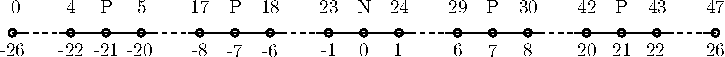
\includegraphics[width=\imsizeL]{asignacion_subportadoras.pdf}
    \caption{Asignación de datos según sus índices a las subportadoras que constituyen un símbolo OFDM.\label{fig:asignacion-subportadoras}}  
\end{figure}

\subsection{Duración temporal del símbolo}
\label{Ss:ch2-tiempo-simbolo}


En función del espacio entre subportadoras, $\Delta_F$, el estándar define distintos intervalos temporales que resultan de interés. Dichos parámetros se resumen en la Tabla \ref{tab:tiempos-formula}. El parámetro $\Delta_F$ es determinado por el espaciamiento entre canales en el dominio de la frecuencia, específicamente es el resultado de dividir entre 64 la separación entre los canales.

En el funcionamiento típico, los canales están espaciados 20 MHz, pero el sistema admite operación en modo mitad de reloj, con espaciamiento de 10 MHz, y cuarto de reloj, con espaciamiento de 5 MHz. La longitud de los intervalos temporales son inversamente proporcionales al espaciamiento entre canales, y sus valores se detallan en la Tabla \ref{tab:tiempos-valor}.

\begin{table}[t]
    \centering{}z
    \begin{tabular}{|l|l|l|}
    \hline
     \thead{Parámetro} & \thead{Significado} & \thead{Fórmula}\\
     \hline
     $T_{FFT}$ & Duración de los intervalos de IFFT y FFT. & $1/\Delta_F$  \\
     $T_{GI}$  & Intervalo de guarda para los símbolos OFDM. & $T_{FFT}/4$      \\
     $T_{SYM}$ & Duración de un símbolo OFDM. & $T_{GI}+T_{FFT}$ \\
     $T_{GI2}$ & Intervalo de guarda para los campos del preámbulo. & $T_{FFT}/2$      \\
     $T_{SHORT}$ & Duración de la primer secuencia de entrenamiento. & $10\times T_{FFT}/4$  \\
     $T_{LONG}$ & Duración de la segunda secuencia de entrenamiento. & $T_{GI2}+2\times T_{FFT}$ \\
     \hline
    \end{tabular}
    \caption{Parámetros temporales y sus fórmulas en función del parámetro $\Delta_F$.\label{tab:tiempos-formula}}
\end{table}

\begin{table}[t]
    \centering{}
    \begin{tabular}{|l|c|c|c|}
    \hline
     \thead{Parámetro} & \thead{Valor con canales\\espaciados 20 MHz}& \thead{Valor con canales\\espaciados 10 MHz} & \thead{Valor con canales\\espaciados 5 MHz} \\
     \hline
     $T_{FFT}$   & $3.2$ \textmu s & $6.4$ \textmu s & $12.8$ \textmu s \\
     $T_{GI}$    & $0.8$ \textmu s & $1.6$ \textmu s & $3.2$ \textmu s \\
     $T_{GI2}$   & $1.6$ \textmu s & $3.2$ \textmu s & $6.4$ \textmu s \\
     $T_{SYM}$   & $4$ \textmu s & $8$ \textmu s & $16$ \textmu s \\
     $T_{SHORT}$ & $8$ \textmu s & $16$ \textmu s & $32$ \textmu s \\
     $T_{LONG}$  & $8$ \textmu s & $16$ \textmu s & $32$ \textmu s \\
     \hline
    \end{tabular}
    \caption{Valores de los parámetros temporales según el espaciamiento entre canales admitidos por el estándar IEEE 802.11.\label{tab:tiempos-valor}}
\end{table}


\subsection{IFFT}
\label{Ss:ch2-ifft}

\begin{figure}{t}
    \centering
    \hfill
    \subcaptionbox{Aplicación de IFFT de 64 puntos.\label{fig:ifft64}}{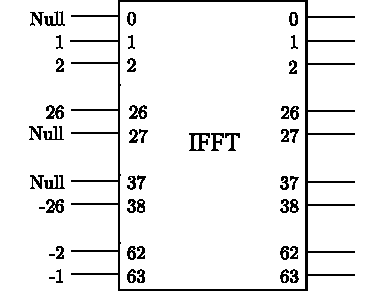
\includegraphics[width=0.5\imsizeL]{IFFT.pdf}}%
    \hfill
    \subcaptionbox{Aplicación de IFFT de 128 puntos.\label{fig:ifft128}}{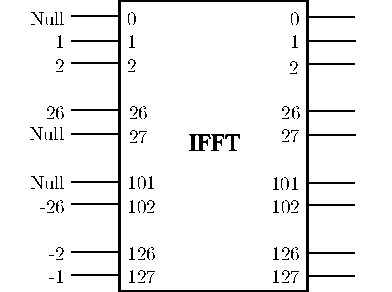
\includegraphics[width=0.5\imsizeL]{IFFT128.pdf}}%
    \caption{Esquema de aplicación de IFFT a una descripción en subportadoras de un símbolo OFDM.\label{fig:ifft}}
    \hfill
\end{figure}

La representación en subportadoras de un símbolo OFDM se transforma al dominio del tiempo con un módulo IFFT. Típicamente, se utilizan módulos IFFT con un número de puntos potencia de 2 necesariamente mayor o igual a 64, en número de puntos utilizados recibe el nombre $N_{FFT}$. Para obtener una correcta transformación del dominio se aplica una operación de desplazamiento, transportando las subportadoras de índice negativo al final del vector de entrada del módulo IFFT. Este desplazamiento se esquematiza en la Figura \ref{fig:ifft}.

En el estándar se define la transformación con $N_{FFT}=64$, sin embargo, aplicando el mismo desplazamiento considerando un valor de $N_{FFFT}$ mayor es posible y resulta en una mayor resolución temporal de la señal. Cabe destacar que independientemente del valor de $N_{FFT}$, la duración temporal de la salida es el valor $T_{FFT}$ definido en la Tabla \ref{tab:tiempos-valor}, y el espacio entre las muestras valdrá $T_S = T_{FFT}/N_{FFT}$.

\subsection{Prefijo cíclico}
\label{Ss:ch2-prefijo}

Al vector resultante de la operación IFFT se le agrega un intervalo de guarda, (GI por sus siglas en inglés), el cual tiene la función de mitigar efectos de interferencia entre símbolos (ISI por sus siglas en inglés). El GI consiste en un prefijo cíclico de la señal temporal, y se construye de la siguiente forma: se toman las últimas $N_{FFT}/4$ muestras de la señal, y se las concatenan al inicio de las $N_{FFT}$ muestras existentes. Este procedimiento se representa gráficamente en la Figura \ref{fig:prefijo}. La inclusión del prefijo cíclico completa la estructura del símbolo OFDM que será transmitido.
\begin{figure}[t]
    \centering{}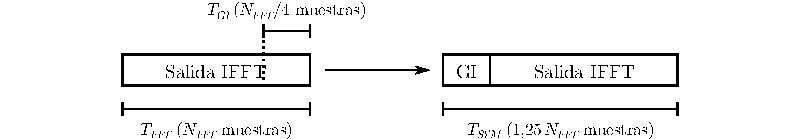
\includegraphics[width=\imsizeL]{prefix.pdf}
    \caption{Diagrama de aplicación de intervalo de guarda a un símbolo OFDM.\label{fig:prefijo}}  
\end{figure}


\section{Estructura de la PPDU}
\label{S:ch2-ppdu}

\begin{figure}[t]
    \centering{}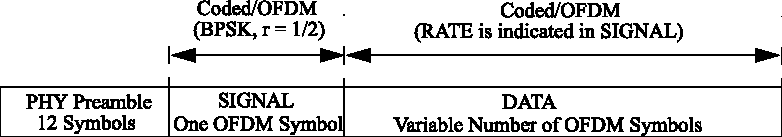
\includegraphics[width=\imsize]{PPDU.pdf}
    \caption{Estructura de alto nivel de una PPDU en el estándar IEEE 802.11.\label{fig:ppdu}}  
\end{figure}

La PPDU consiste en una secuencia de símbolos OFDM que transmiten un mensaje a través de la capa física, la cual se describe en la Figura \ref*{fig:ppdu}, esta incorpora a un mensaje la información requerida para detección, sincronismo, demodulación, y decodificación del mismo. Los campos que la constituyen son los siguientes:

\begin{enumerate}
    \item PHY Preamble: secuencia de símbolos OFDM predeterminados utilizados para detección, sincronismo, y estimación del canal.
    \item SIGNAL: símbolo OFDM que transmite la información necesaria para la recepción de DATA a través de los campos LENGTH y RATE. Siempre es modulado en BPSK y codificado a tasa 1/2.
    \item DATA: número variable de símbolos OFDM que transmiten la información del mensaje propiamente dicha, el número de símbolos es informado por LENGTH, y la modulación de cada subportadora y tasa del código de correción de errores utilizados son determinadas únivocamente por RATE.
\end{enumerate}

El campo PHY Preamble cumple un rol fundamental en lo que hace a la detección y sincronismo tanto en tiempo como en frecuencia en el receptor,  por lo que se hará énfasis en su estructura a lo largo de este trabajo. En cambio, las funciones y estructuras de los campos SIGNAL y DATA exceden el alcance del proyecto, por lo que no se estudiarán en mayor detalle.

\section{PHY Preamble}
\label{S:ch2-preambulo}

El preámbulo es una forma de onda predeterminada transmitida al inicio de cada PPDU. Éste consiste en dos secuencias, las cuales se construyen de forma similar a otros símbolos pero en lugar de contener datos y tonos pilotos las 52 subportadoras son asignadas valores predefinidos. Las dos secuencias reciben el nombre de secuencia de entrenamiento de símbolos cortos y secuencia de entrenamiento de símbolos largos, y las asignaciones de subportadoras usadas para construirlas son definidas por los vectores $S$ y $L$ respectivamente:
\begin{align}
    &\begin{aligned}
        S_{-26,26} = \sqrt{13/6}\, 
        [&0 ,\,  0   ,\, 1+j ,\,  0   ,\, 0 ,\,  0   ,\, -1-j ,\,  0   ,\, 0 ,\, 0   ,\, 1+j ,\, 0   ,\, 0 ,\, 
         0 ,\, -1-j ,\, 0   ,\,  0   ,\, 0 ,\\ 
         &-1-j ,\,  0   ,\,  0   ,\, 0 ,\, 1+j ,\, 0   ,\, 0   ,\, 0 ,\, 0 ,\,
         0 ,\,  0   ,\, 0   ,\, -1-j ,\, 0 ,\,  0   ,\,  0   ,\, -1-j ,\\ 
         &0 ,\, 0   ,\, 0   ,\, 1+j ,\, 0 ,\, 
         0 ,\,  0   ,\, 1+j ,\,  0   ,\, 0 ,\,  0   ,\,  1+j ,\,  0   ,\, 0 ,\, 0   ,\, 1+j ,\, 0   ,\, 0]
    \end{aligned}\label{eq:def-S}\\
    &
    \begin{aligned}
        L_{-26,26} = 
        [&1,\, 1,\, -1,\, -1,\, 1,\, 1,\, -1,\, 1,\, -1,\, 1,\, 1,\, 1,\, 1,\, 1,\, 1,\, -1,\, -1, 1,\, 1,\, -1,\, 1,\, -1,\, 1,\\& 1,\, 1,\, 1,\, 
        0,\,
        1,\, -1,\, -1,\, 1,\, 1,\, -1,\, 1,\, -1,\, 1, -1,\, -1,\, -1,\, -1,\, -1,\, 1,\, 1,\, -1,\\& -1,\, 1,\, -1,\, 1,\, -1,\, 1,\, 1,\, 1,\, 1]
    \end{aligned}\label{eq:def-L}
\end{align}
\begin{figure}[t]
    \centering{}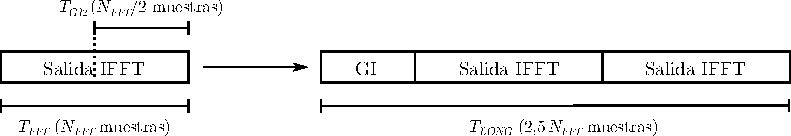
\includegraphics[width=\imsizeL]{training_symbol.pdf}
    \caption{Diagrama de aplicación de intervalo de guarda a una secuencia de entrenamiento del preámbulo.\label{fig:training-symbol}}  
\end{figure}

A diferencia de los símbolos OFDM pertenecientes a los campos SIGNAL y DATA, las secuencias de entrenamiento tienen el doble de duración, la cual es establecida por los valores $T_{SHORT}$ y $T_{LONG}$ registrados en la Tabla \ref{tab:tiempos-valor}. Su intervalo de guarda también tiene el doble de duración, definida por $T_{GI2}$. El procedimiento para construir una secuencia de entrenamiento a partir de la salida del módulo IFFT se describe en la Figura \ref{fig:training-symbol}.

\subsection{Secuencia de entrenamiento de símbolos cortos}
\label{Ss:ch2-short}
%\begin{equation}\label{eq:def-S}
%    \begin{aligned}
%    S_{-26,26} = \sqrt{13/6}\, 
%    [0 ,\,  0   ,\, 1+j ,\,  0   ,\, 0 ,\,  0   ,\, -1-j ,\,  0   ,\, 0 ,\, 0   ,\, 1+j ,\, 0   ,\, 0 ,\, 
%     0 ,\, -1-j ,\, 0   ,\,  0   ,\, 0 ,\\ -1-j ,\,  0   ,\,  0   ,\, 0 ,\, 1+j ,\, 0   ,\, 0   ,\, 0 ,\, 0 ,\,
%     0 ,\,  0   ,\, 0   ,\, -1-j ,\, 0 ,\,  0   ,\,  0   ,\, -1-j ,\\ 0 ,\, 0   ,\, 0   ,\, 1+j ,\, 0 ,\, 
%     0 ,\,  0   ,\, 1+j ,\,  0   ,\, 0 ,\,  0   ,\,  1+j ,\,  0   ,\, 0 ,\, 0   ,\, 1+j ,\, 0   ,\, 0]
%    \end{aligned}
%\end{equation}

\begin{figure}[t]
    \centering{}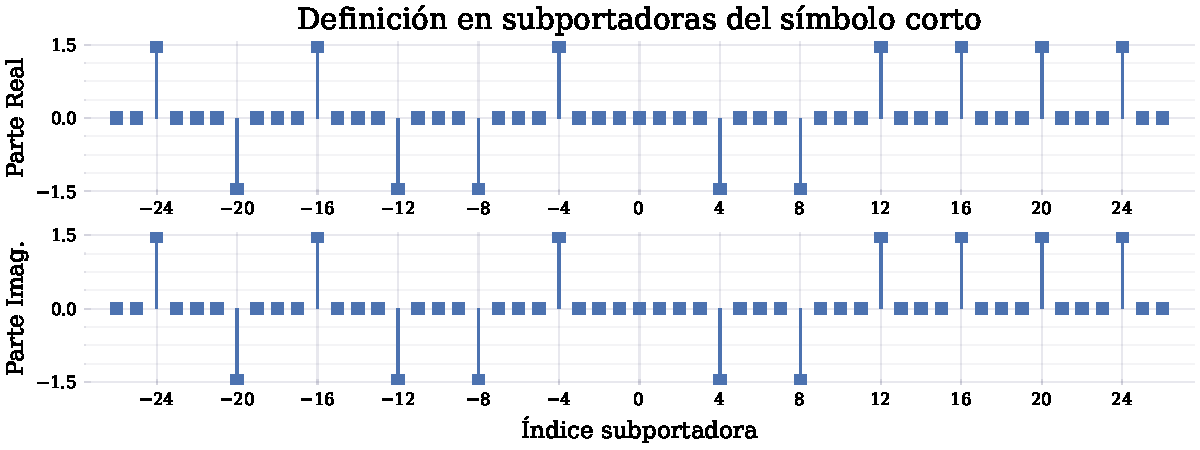
\includegraphics[width=\imsize]{short_sc.pdf}
    \caption{Asignación de subportadoras para la construcción de la secuencia de entrenamiento de símbolos cortos.\label{fig:short-sc}}  
\end{figure}
\begin{figure}[t]
    \centering{}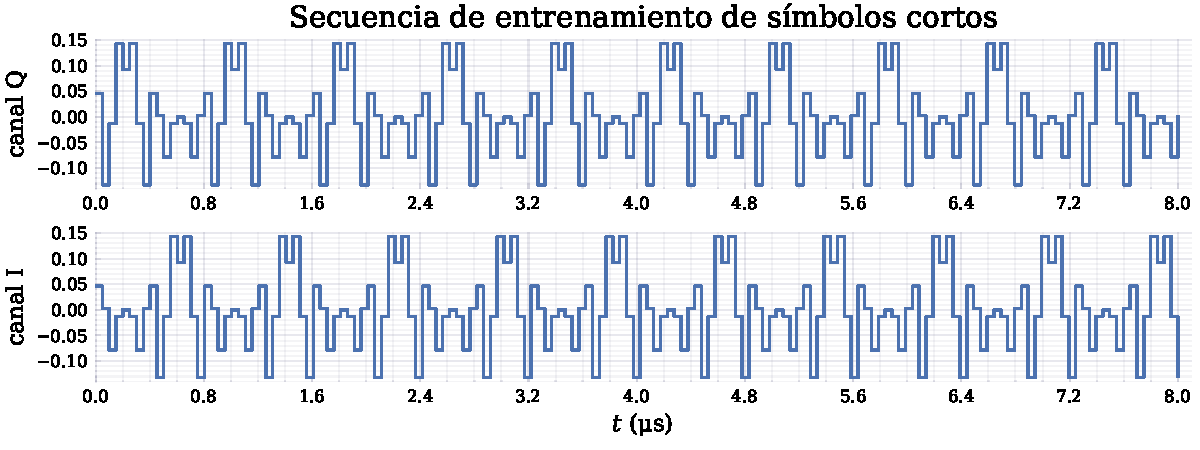
\includegraphics[width=\imsize]{short_time.pdf}
    \caption{Secuencia de entrenamiento de símbolos cortos en el dominio temporal, usando $T_{SHORT} = 8$ \textmu s y una IFFT de 64 puntos.\label{fig:short-time}}  
\end{figure}

La secuencia de entrenamiento de símbolos cortos representa la primera mitad del preámbulo, construída a partir de el resultado de aplicar la IFFT a la secuencia $S$ definida en la Ecuación \ref{eq:def-S}. Esta secuencia asigna valores complejos únicamente a subportadoras con índices múltiplos de 4, la secuencia se grafica en la Figura \ref{fig:short-sc}.

Aplicar la IFFT a $S$ y agregar el intervalo de guarda produce una señal con un período de duración $T_{FFT}/4$, el cual recibe el nombre de símbolo corto. La secuencia de entrenamiento de símbolos cortos contiene 10 de estos símbolos y es graficada en la Figura \ref{fig:short-time}. Ésta secuencia cumple la función de facilitar la detección de la señal entrante en el receptor, así como permitir algoritmos preliminares de sincronismo, y es de vital importancia para este proyecto.

\subsection{Secuencia de entrenamiento de símbolos largos}
\label{Ss:ch2-long}
%\begin{equation}\label{eq:def-L}
%    \begin{aligned}
%    L = 
%    [1,\, 1,\, -1,\, -1,\, 1,\, 1,\, -1,\, 1,\, -1,\, 1,\, 1,\, 1,\, 1,\, 1,\, 1,\, -1,\, -1,\\
%    1,\, 1,\, -1,\, 1,\, -1,\, 1,\, 1,\, 1,\, 1,\, 
%    0,\,
%    1,\, -1,\, -1,\, 1,\, 1,\, -1,\, 1,\, -1,\, 1,
%    \\ -1,\, -1,\, -1,\, -1,\, -1,\, 1,\, 1,\, -1,\, -1,\, 1,\, -1,\, 1,\, -1,\, 1,\, 1,\, 1,\, 1]
%    \end{aligned}
%\end{equation}
    
\begin{figure}[t]
    \centering{}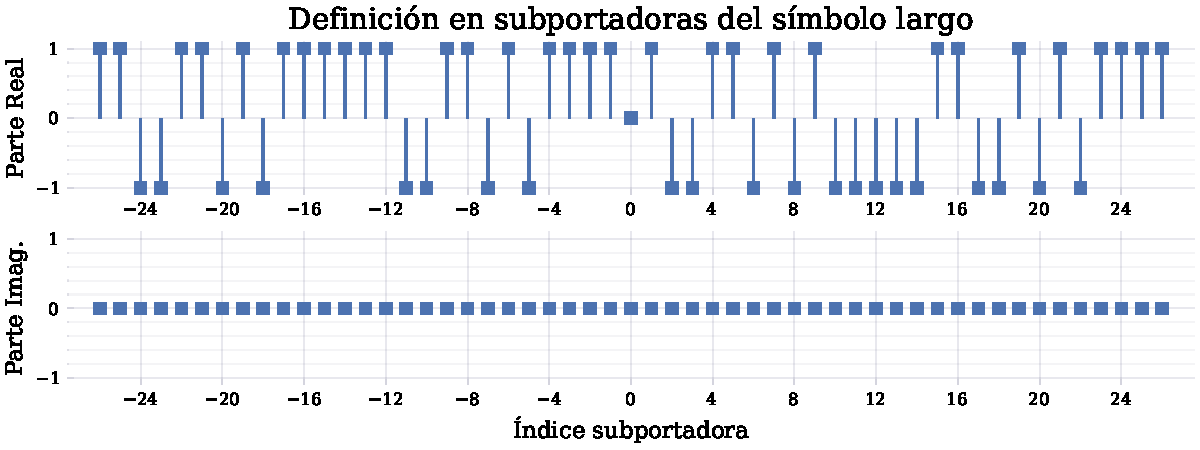
\includegraphics[width=\imsize]{long_sc.pdf}
    \caption{Asignación de subportadoras para la construcción de la secuencia de entrenamiento de símbolos largos.\label{fig:long-sc}}
\end{figure}
\begin{figure}[t]
    \centering{}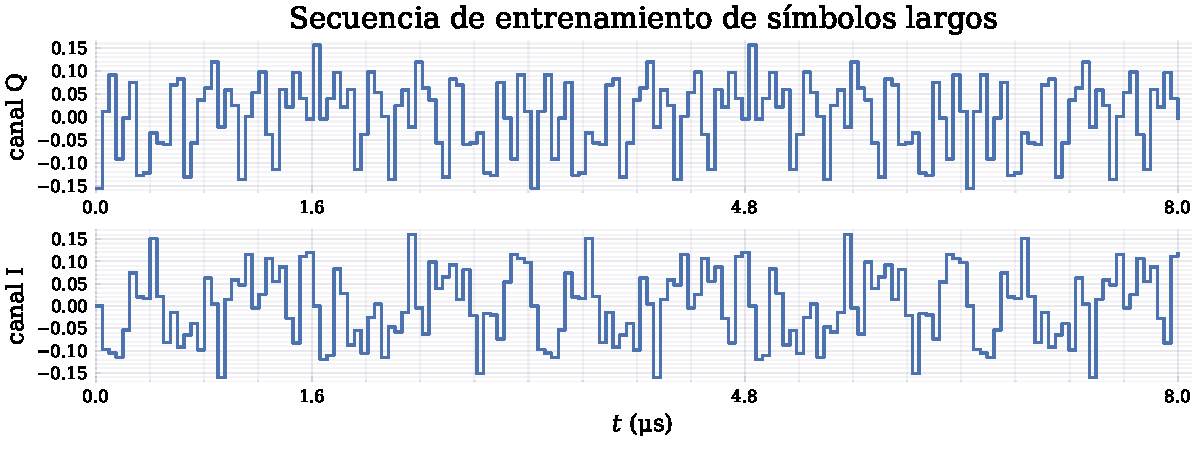
\includegraphics[width=\imsize]{long_time.pdf}
    \caption{Secuencia de entrenamiento de símbolos largos en el dominio temporal, usando $T_{LONG} = 8$ \textmu s y una IFFT de 64 puntos..\label{fig:long-time}}  
\end{figure}

La secuencia de entrenamiento de símbolos cortos representa la segunda mitad del preámbulo. La IFFT es aplicada a la secuencia $L$ definida en la Ecuación \ref{eq:def-L} la cual se grafica en la Figura \ref{fig:long-sc}. A diferencia de $S$, esta asigna valores a todas las subportadoras.

En este caso, aplicar la IFFT produce el símbolo largo de duración $T_{FFT}$, y la secuencia de entrenamiento de símbolos largos la cual es graficada en la Figura \ref{fig:long-time} consiste en 2.5 de estos símbolos. Sus funciones incluyen permitir algoritmos de sincronismo fino en el receptor, así como funciones de estimación de la respuesta al impulso del canal.


\section{Resumen del capítulo}

En el capítulo se resumieron las características de las señales que emplean OFDM de acuerdo con el estándar IEEE 802.11 que son necesarias para poder llevar adelante el proyecto. Se detalla el procedimiento para construir un símbolo OFDM a partir de una secuencia de coordenadas resultantes de una constelación de modulación y como estos símbolos se organizan para formar una PPDU.

Se presta particular atención al campo PHY Preamble, específicamente a su primer mitad, la secuencia de de entrenamiento de símbolos cortos. Conocer la forma y las propiedades de esta secuencia de entrenamiento se permite implementar algoritmos de detección y sincronismo, tal como se describirá en los capítulos siguientes.

%%% Local Variables: 
%%% mode: latex
%%% TeX-master: "template"
%%% End: 
